\documentclass[11pt,a4paper]{article}

\usepackage[margin=2cm]{geometry}
\usepackage[T1]{fontenc}
\usepackage{lmodern}
\usepackage{amsmath,amssymb}
\usepackage{booktabs}
\usepackage{listings}
\usepackage{tikz}
\usetikzlibrary{arrows.meta}

\lstset{
  language=C,
  basicstyle=\ttfamily\small,
  keywordstyle=\bfseries,
  numbers=left,
  numberstyle=\small,
  firstnumber=0,
  columns=fullflexible,
  keepspaces=true,
  morekeywords={assert,goto}
}

% let TeX stretch spaces a bit instead of letting lines run into the margin
\setlength{\emergencystretch}{2em}

% scale a picture down to the line width if it is wider, otherwise keep it as is
\newsavebox{\fitboxcontent}
\newenvironment{fitbox}
  {\begin{lrbox}{\fitboxcontent}}
  {\end{lrbox}%
   \ifdim\wd\fitboxcontent>\linewidth
     \resizebox{\linewidth}{!}{\usebox{\fitboxcontent}}%
   \else
     \usebox{\fitboxcontent}%
   \fi}

% abstract states; \allowbreak lets a state wrap after a comma in running text
% abstract state: pc, x, i (Exercise 1)
\newcommand{\st}[3]{$\mathit{pc}\colon #1,\allowbreak\ x\colon #2,\allowbreak\ i\colon #3$}
% abstract state: pc, x, y, z (Exercise 2)
\newcommand{\stz}[4]{$\mathit{pc}\colon #1,\allowbreak\ x\colon #2,\allowbreak\ y\colon #3,\allowbreak\ z\colon #4$}
% abstract state: pc, x, y, i (Exercise 3)
\newcommand{\sti}[4]{$\mathit{pc}\colon #1,\allowbreak\ x\colon #2,\allowbreak\ y\colon #3,\allowbreak\ i\colon #4$}
\newcommand{\itv}[2]{[#1,\,#2]}
\newcommand{\ninf}{-\infty}
\newcommand{\pinf}{+\infty}
\newcommand{\INTd}{\mathit{INT}_d}
\newcommand{\INTp}{\mathit{INT}'}

\title{VU Advanced Software Engineering (194.187, WS2026)\\
       Sheet 1: Abstract Interpretation}
\author{Kristijan Todorovic}
\date{}

\begin{document}
\maketitle

\section*{Exercise 1: Widening}

\begin{lstlisting}
void verify_with_widening(int x) {
    if (x >= 0)
        x = -1;
    int i = x;
    if (i < 1) {
        i = i + 2;
        x = x * 2;
        goto 4;
    }
    assert(x < i);
}
\end{lstlisting}

\subsection*{Setup (as in the lecture)}

\begin{itemize}
  \item \textbf{Abstract domain:} the standard interval domain
        $\{[a,b] \mid a \le b,\ a \in \mathbb{Z}\cup\{\ninf\},\ b \in \mathbb{Z}\cup\{\pinf\}\} \cup \{\bot\}$,
        ordered by inclusion. An abstract state maps $\mathit{pc}$ to a line and each program
        variable to an interval. The parameter \texttt{x} is unknown at entry, so
        $x\colon\itv{\ninf}{\pinf}$. Since \texttt{i} is not assigned before line~3, $i\colon\bot$.
  \item \textbf{Transformers:}
        \begin{itemize}
          \item $i = x$: \ $i$ gets the interval of $x$.
          \item $i = i + 2$: \ $\itv{a}{b} + 2 = \itv{a+2}{b+2}$.
          \item $x = x * 2$: \ $\itv{a}{b} \cdot 2 = \itv{2a}{2b}$.
          \item Conditions: intersect the interval with the condition, e.g.\
                $i < 1$ gives $\itv{a}{b} \sqcap \itv{\ninf}{0}$ and
                $i \ge 1$ gives $\itv{a}{b} \sqcap \itv{1}{\pinf}$.
                An empty intersection is $\bot$, which means that the branch is infeasible.
        \end{itemize}
  \item \textbf{Join} (states at the same program label):
        $\itv{a}{b} \sqcup \itv{c}{d} = \itv{\min(a,c)}{\max(b,d)}$, and $\bot$ is neutral.
  \item \textbf{Widening} (applied after every \texttt{goto}, where we previously used JOIN, as $\mathit{old} \mathbin{\nabla} \mathit{new}$):
        \begin{gather*}
          \itv{a}{b} \mathbin{\nabla} \bot = \itv{a}{b}, \qquad
          \bot \mathbin{\nabla} \itv{a}{b} = \itv{a}{b}, \\
          \itv{a}{b} \mathbin{\nabla} \itv{c}{d} =
          \big[\, c < a \;?\; \ninf : a,\ \ b < d \;?\; \pinf : b \,\big].
        \end{gather*}
\end{itemize}

\subsection*{Iteration}

\paragraph{Before the loop.}
At line~1 the state is \st{1}{\itv{\ninf}{\pinf}}{\bot}.
\begin{itemize}
  \item Branch $x \ge 0$: \st{2}{\itv{0}{\pinf}}{\bot}. After $x = -1$ we get \st{3}{\itv{-1}{-1}}{\bot}.
  \item Branch $x < 0$: \st{3}{\itv{\ninf}{-1}}{\bot}.
  \item JOIN at line 3: $\itv{-1}{-1} \sqcup \itv{\ninf}{-1} = \itv{\ninf}{-1}$, so we get \st{3}{\itv{\ninf}{-1}}{\bot}.
  \item $i = x$: \st{4}{\itv{\ninf}{-1}}{\itv{\ninf}{-1}}.
\end{itemize}

\paragraph{Loop iteration 1.}
\begin{itemize}
  \item $i \ge 1$: $\itv{\ninf}{-1} \sqcap \itv{1}{\pinf} = \bot$, so we get \st{9}{\itv{\ninf}{-1}}{\bot} (infeasible).
  \item $i < 1$: \st{5}{\itv{\ninf}{-1}}{\itv{\ninf}{-1}}.
  \item $i = i + 2$: \st{6}{\itv{\ninf}{-1}}{\itv{\ninf}{1}}.
  \item $x = x * 2$: \st{7}{\itv{\ninf}{-2}}{\itv{\ninf}{1}}.
  \item \texttt{goto 4}: \st{4}{\itv{\ninf}{-2}}{\itv{\ninf}{1}}.
  \item WIDEN with the previous state at line 4:
        \begin{align*}
          x\colon\ & \itv{\ninf}{-1} \mathbin{\nabla} \itv{\ninf}{-2} = \itv{\ninf}{-1}
            && (\ninf \nless \ninf \text{ and } -1 \nless -2), \\
          i\colon\ & \itv{\ninf}{-1} \mathbin{\nabla} \itv{\ninf}{1} = \itv{\ninf}{\pinf}
            && (-1 < 1).
        \end{align*}
        The result is \st{4}{\itv{\ninf}{-1}}{\itv{\ninf}{\pinf}}.
\end{itemize}

\paragraph{Loop iteration 2.}
\begin{itemize}
  \item $i \ge 1$: \st{9}{\itv{\ninf}{-1}}{\itv{1}{\pinf}}.
  \item $i < 1$: \st{5}{\itv{\ninf}{-1}}{\itv{\ninf}{0}}.
  \item $i = i + 2$: \st{6}{\itv{\ninf}{-1}}{\itv{\ninf}{2}}.
  \item $x = x * 2$: \st{7}{\itv{\ninf}{-2}}{\itv{\ninf}{2}}.
  \item \texttt{goto 4}: \st{4}{\itv{\ninf}{-2}}{\itv{\ninf}{2}}.
  \item WIDEN:
        $x\colon \itv{\ninf}{-1} \mathbin{\nabla} \itv{\ninf}{-2} = \itv{\ninf}{-1}$ and
        $i\colon \itv{\ninf}{\pinf} \mathbin{\nabla} \itv{\ninf}{2} = \itv{\ninf}{\pinf}$.
        The result is \st{4}{\itv{\ninf}{-1}}{\itv{\ninf}{\pinf}}. This equals the previous
        state at line~4, so we have reached a \textbf{fixed point}.
\end{itemize}

\paragraph{Exit (line 9).}
JOIN of all states that reach line~9:
\[
  x\colon \itv{\ninf}{-1} \sqcup \itv{\ninf}{-1} = \itv{\ninf}{-1}, \qquad
  i\colon \bot \sqcup \itv{1}{\pinf} = \itv{1}{\pinf}.
\]
The state at line 9 is \st{9}{\itv{\ninf}{-1}}{\itv{1}{\pinf}}.

\begin{center}
\begin{tabular}{@{}lll@{}}
  \toprule
  State at line 4 & $x$ & $i$ \\
  \midrule
  initial (after $i = x$)        & $\itv{\ninf}{-1}$ & $\itv{\ninf}{-1}$ \\
  after iteration 1 (widened)    & $\itv{\ninf}{-1}$ & $\itv{\ninf}{\pinf}$ \\
  after iteration 2 (widened)    & $\itv{\ninf}{-1}$ & $\itv{\ninf}{\pinf}$ \quad (fixed point) \\
  \bottomrule
\end{tabular}
\end{center}

\newpage
\subsection*{Abstract control flow graph}

Solid edges are labelled with the executed instruction or branch condition.
Dashed edges are labelled JOIN or WIDEN.

\begin{center}
\begin{fitbox}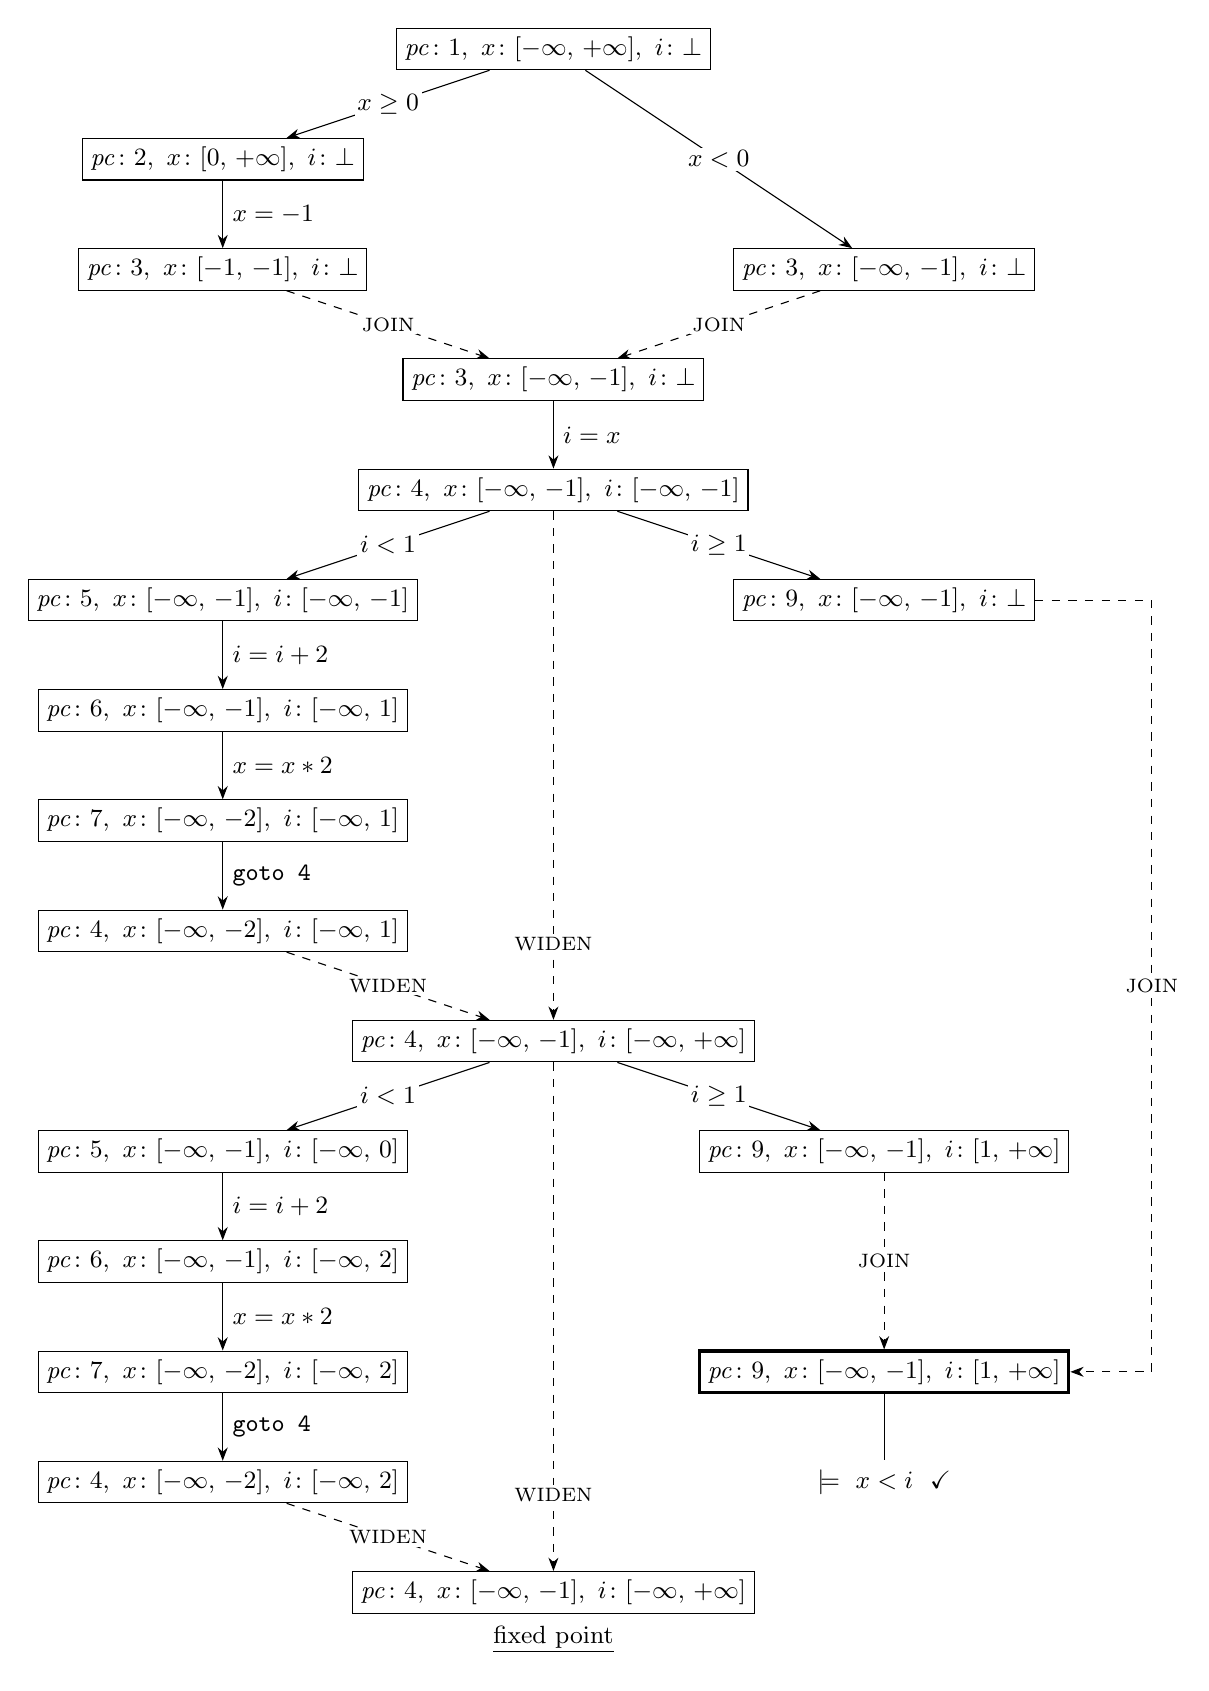
\begin{tikzpicture}[
    state/.style={draw, rectangle, align=center, inner sep=3pt, font=\small},
    instr/.style={-{Stealth}},
    meta/.style={-{Stealth}, dashed},
    lbl/.style={font=\small},
    mlbl/.style={font=\scriptsize, fill=white, inner sep=1pt}
  ]

  % before the loop
  \node[state] (s1)  at (0,0)       {\st{1}{\itv{\ninf}{\pinf}}{\bot}};
  \node[state] (s2)  at (-4.2,-1.4) {\st{2}{\itv{0}{\pinf}}{\bot}};
  \node[state] (s3a) at (-4.2,-2.8) {\st{3}{\itv{-1}{-1}}{\bot}};
  \node[state] (s3b) at (4.2,-2.8)  {\st{3}{\itv{\ninf}{-1}}{\bot}};
  \node[state] (s3)  at (0,-4.2)    {\st{3}{\itv{\ninf}{-1}}{\bot}};
  \node[state] (s4)  at (0,-5.6)    {\st{4}{\itv{\ninf}{-1}}{\itv{\ninf}{-1}}};

  % loop iteration 1
  \node[state] (s5)  at (-4.2,-7)    {\st{5}{\itv{\ninf}{-1}}{\itv{\ninf}{-1}}};
  \node[state] (s9a) at (4.2,-7)     {\st{9}{\itv{\ninf}{-1}}{\bot}};
  \node[state] (s6)  at (-4.2,-8.4)  {\st{6}{\itv{\ninf}{-1}}{\itv{\ninf}{1}}};
  \node[state] (s7)  at (-4.2,-9.8)  {\st{7}{\itv{\ninf}{-2}}{\itv{\ninf}{1}}};
  \node[state] (s4b) at (-4.2,-11.2) {\st{4}{\itv{\ninf}{-2}}{\itv{\ninf}{1}}};
  \node[state] (s4w) at (0,-12.6)    {\st{4}{\itv{\ninf}{-1}}{\itv{\ninf}{\pinf}}};

  % loop iteration 2
  \node[state] (t5)  at (-4.2,-14)   {\st{5}{\itv{\ninf}{-1}}{\itv{\ninf}{0}}};
  \node[state] (s9b) at (4.2,-14)    {\st{9}{\itv{\ninf}{-1}}{\itv{1}{\pinf}}};
  \node[state] (t6)  at (-4.2,-15.4) {\st{6}{\itv{\ninf}{-1}}{\itv{\ninf}{2}}};
  \node[state] (t7)  at (-4.2,-16.8) {\st{7}{\itv{\ninf}{-2}}{\itv{\ninf}{2}}};
  \node[state] (t4b) at (-4.2,-18.2) {\st{4}{\itv{\ninf}{-2}}{\itv{\ninf}{2}}};
  \node[state] (s4f) at (0,-19.6)    {\st{4}{\itv{\ninf}{-1}}{\itv{\ninf}{\pinf}}};
  \node[lbl, below=1pt] at (s4f.south) {\underline{fixed point}};

  % exit
  \node[state, very thick] (s9) at (4.2,-16.8) {\st{9}{\itv{\ninf}{-1}}{\itv{1}{\pinf}}};
  \node[lbl] (chk) at (4.2,-18.2) {$\models\ x < i$ \ \checkmark};

  % edges before the loop
  \draw[instr] (s1) -- node[mlbl, font=\small]  {$x \ge 0$} (s2);
  \draw[instr] (s1) -- node[mlbl, font=\small] {$x < 0$}   (s3b);
  \draw[instr] (s2) -- node[lbl, right] {$x = -1$} (s3a);
  \draw[meta]  (s3a) -- node[mlbl] {JOIN} (s3);
  \draw[meta]  (s3b) -- node[mlbl] {JOIN} (s3);
  \draw[instr] (s3) -- node[lbl, right] {$i = x$} (s4);

  % edges loop iteration 1
  \draw[instr] (s4) -- node[mlbl, font=\small]  {$i < 1$}   (s5);
  \draw[instr] (s4) -- node[mlbl, font=\small] {$i \ge 1$} (s9a);
  \draw[instr] (s5) -- node[lbl, right] {$i = i + 2$} (s6);
  \draw[instr] (s6) -- node[lbl, right] {$x = x * 2$} (s7);
  \draw[instr] (s7) -- node[lbl, right] {\texttt{goto 4}} (s4b);
  \draw[meta]  (s4b) -- node[mlbl] {WIDEN} (s4w);
  \draw[meta]  (s4)  -- node[mlbl, pos=0.85] {WIDEN} (s4w);

  % edges loop iteration 2
  \draw[instr] (s4w) -- node[mlbl, font=\small]  {$i < 1$}   (t5);
  \draw[instr] (s4w) -- node[mlbl, font=\small] {$i \ge 1$} (s9b);
  \draw[instr] (t5) -- node[lbl, right] {$i = i + 2$} (t6);
  \draw[instr] (t6) -- node[lbl, right] {$x = x * 2$} (t7);
  \draw[instr] (t7) -- node[lbl, right] {\texttt{goto 4}} (t4b);
  \draw[meta]  (t4b) -- node[mlbl] {WIDEN} (s4f);
  \draw[meta]  (s4w) -- node[mlbl, pos=0.85] {WIDEN} (s4f);

  % edges exit
  \draw[meta]  (s9a.east) -- (7.6,-7) |- node[mlbl, pos=0.25] {JOIN} (s9.east);
  \draw[meta]  (s9b) -- node[mlbl] {JOIN} (s9);
  \draw (s9) -- (chk);
\end{tikzpicture}\end{fitbox}
\end{center}

\subsection*{What does the analysis reveal about safety?}

The abstract state at line~9, i.e.\ at the assertion, is
\[
  \mathit{pc}\colon 9,\quad x \in \itv{\ninf}{-1},\quad i \in \itv{1}{\pinf}.
\]
Every value of $x$ is at most $-1$ and every value of $i$ is at least $1$. So
$x \le -1 < 1 \le i$, and \texttt{x < i} holds in every concrete state described by the
abstract state:
\[
  P_{\mathit{int}} \models (x < i) \quad \checkmark
\]
Abstract interpretation with the interval domain and widening is sound. The computed
over-approximation contains all reachable states, so the assertion can never fail and
\texttt{verify\_with\_widening} is \textbf{safe}. The analysis verifies it.

Widening loses precision here: at the loop head the upper bound of $i$ is pushed to
$\pinf$. However, the bound we need is kept for two reasons:
\begin{itemize}
  \item The upper bound of $x$ does not grow ($x$ only gets smaller, from $-1$ to $-2$),
        so widening keeps $x \le -1$.
  \item The lower bound of $i$ at line~9 comes from the loop exit condition $i \ge 1$, not
        from the widened loop invariant.
\end{itemize}

\medskip
\noindent\textit{Remark.} As in the lecture, we assume mathematical (unbounded) integers.
With 32-bit machine integers, \texttt{x * 2} overflows for $x < \texttt{INT\_MIN}/2$,
which is undefined behaviour in C. This case is outside the abstract semantics used here.

%======================================================================
\newpage
\section*{Exercise 2: Modified Interval Domain}

\begin{lstlisting}
void check_verified(unsigned int y) {
    unsigned int x = 3;
    unsigned int z = x;
    if (y <= 1) {
        x = y + 1;
        z = x * x;
    }
    assert(x != 0 && z < 5);
}
\end{lstlisting}

\subsection*{The domain $\INTd$}

\[
  \INTd = \{\, [a,b] \mid a \ge 0,\ a \le b \le a + 2 \,\} \cup \{\bot,\ \itv{0}{\pinf}\}
\]
(we read $[a,b]$ as an interval, so $a \le b$). Apart from the top element $\itv{0}{\pinf}$,
$\INTd$ only contains non-negative intervals of \emph{width at most 2}, i.e.\ intervals
that contain at most three values. Elements are ordered by inclusion, as in the standard
interval domain.

\begin{itemize}
  \item \textbf{Abstraction.} A non-empty set of values with smallest value $l$ and largest
        value $u$ is mapped to the smallest element of $\INTd$ that contains it:
        \[
          \alpha_d(\itv{l}{u}) =
          \begin{cases}
            \itv{l}{u}    & \text{if } u - l \le 2 \text{ and } u \neq \pinf,\\
            \itv{0}{\pinf} & \text{otherwise.}
          \end{cases}
        \]
        For example, $\itv{1}{4}$ (width 3) and $\itv{2}{\pinf}$ cannot be represented and
        both become $\itv{0}{\pinf}$.
  \item \textbf{Transformers.} Compute the result as in the standard interval domain and
        then apply $\alpha_d$. For example, $x = y + 1$ maps $\itv{a}{b}$ to
        $\alpha_d(\itv{a+1}{b+1})$, $z = x * x$ maps $\itv{a}{b}$ to $\alpha_d(\itv{a^2}{b^2})$
        (for $a \ge 0$), and a condition intersects the interval with the condition and then
        applies $\alpha_d$.
  \item \textbf{Join.} $\itv{a}{b} \sqcup_d \itv{c}{d} = \alpha_d(\itv{\min(a,c)}{\max(b,d)})$,
        and $\bot$ is neutral.
\end{itemize}

$\INTd$ has finite height: a strictly increasing chain is at most
$\bot \sqsubset \itv{a}{a} \sqsubset \itv{a}{a+1} \sqsubset \itv{a}{a+2} \sqsubset \itv{0}{\pinf}$,
so no widening is needed. (The program has no loop anyway.)

\subsection*{Iteration}

The parameter \texttt{y} is an arbitrary unsigned value, so $y\colon\itv{0}{\pinf}$ at entry.
The variables \texttt{x} and \texttt{z} are not assigned yet, so they are $\bot$.
\begin{itemize}
  \item \stz{1}{\bot}{\itv{0}{\pinf}}{\bot}.
  \item $x = 3$: \stz{2}{\itv{3}{3}}{\itv{0}{\pinf}}{\bot}.
  \item $z = x$: \stz{3}{\itv{3}{3}}{\itv{0}{\pinf}}{\itv{3}{3}}.
  \item Branch $y \le 1$: \stz{4}{\itv{3}{3}}{\itv{0}{1}}{\itv{3}{3}}.
        \begin{itemize}
          \item $x = y + 1$: $\itv{0}{1} + 1 = \itv{1}{2}$, so \stz{5}{\itv{1}{2}}{\itv{0}{1}}{\itv{3}{3}}.
          \item $z = x * x$: $\itv{1}{2} \cdot \itv{1}{2} = \itv{1}{4}$ has width 3, so
                $\alpha_d(\itv{1}{4}) = \itv{0}{\pinf}$ and we get
                \stz{7}{\itv{1}{2}}{\itv{0}{1}}{\itv{0}{\pinf}}.
        \end{itemize}
  \item Branch $y > 1$: $\itv{0}{\pinf} \sqcap \itv{2}{\pinf} = \itv{2}{\pinf}$, and
        $\alpha_d(\itv{2}{\pinf}) = \itv{0}{\pinf}$, so we get
        \stz{7}{\itv{3}{3}}{\itv{0}{\pinf}}{\itv{3}{3}}.
  \item JOIN at line 7:
        \begin{align*}
          x\colon\ & \itv{1}{2} \sqcup_d \itv{3}{3} = \alpha_d(\itv{1}{3}) = \itv{1}{3}, \\
          y\colon\ & \itv{0}{1} \sqcup_d \itv{0}{\pinf} = \itv{0}{\pinf}, \\
          z\colon\ & \itv{0}{\pinf} \sqcup_d \itv{3}{3} = \itv{0}{\pinf}.
        \end{align*}
        The result is \stz{7}{\itv{1}{3}}{\itv{0}{\pinf}}{\itv{0}{\pinf}}.
\end{itemize}

\subsection*{Abstract control flow graph}

\begin{center}
\begin{fitbox}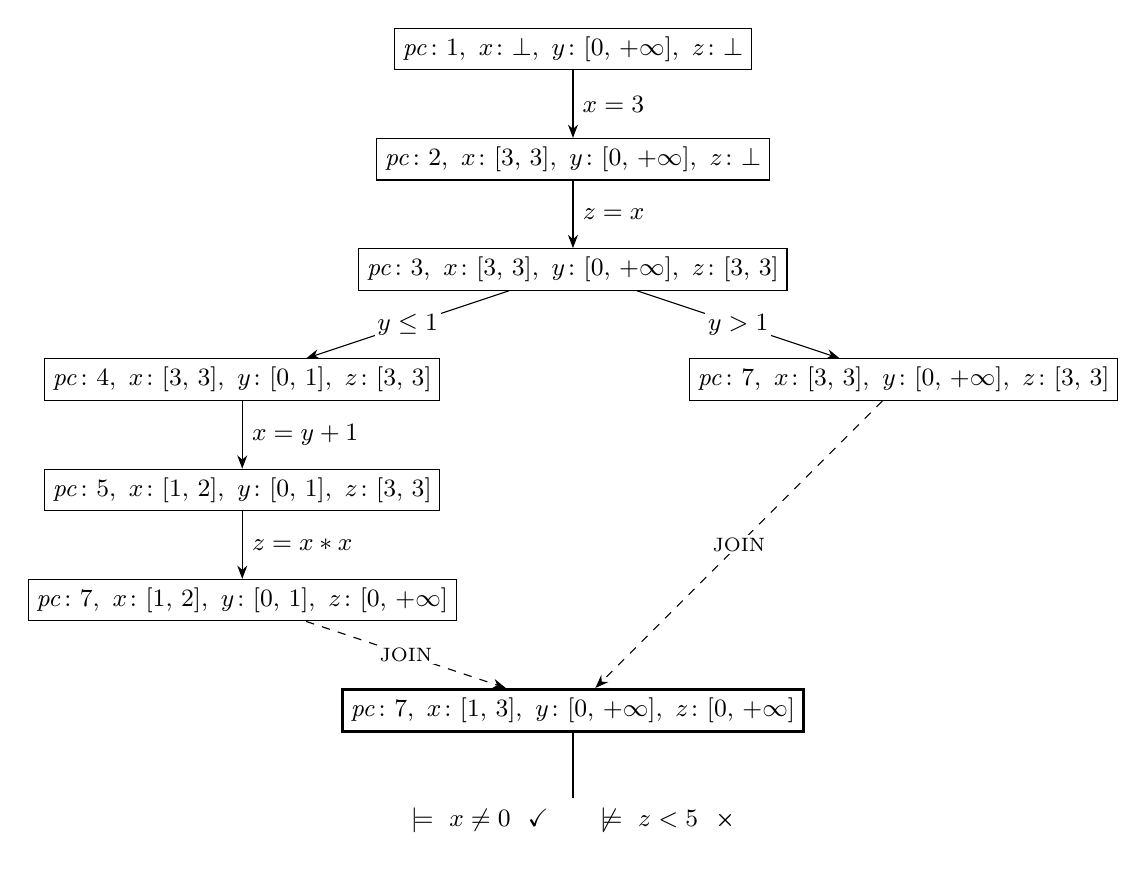
\begin{tikzpicture}[
    state/.style={draw, rectangle, align=center, inner sep=3pt, font=\small},
    instr/.style={-{Stealth}},
    meta/.style={-{Stealth}, dashed},
    lbl/.style={font=\small},
    mlbl/.style={font=\scriptsize, fill=white, inner sep=1pt}
  ]

  \node[state] (s1)  at (0,0)       {\stz{1}{\bot}{\itv{0}{\pinf}}{\bot}};
  \node[state] (s2)  at (0,-1.4)    {\stz{2}{\itv{3}{3}}{\itv{0}{\pinf}}{\bot}};
  \node[state] (s3)  at (0,-2.8)    {\stz{3}{\itv{3}{3}}{\itv{0}{\pinf}}{\itv{3}{3}}};
  \node[state] (s4)  at (-4.2,-4.2) {\stz{4}{\itv{3}{3}}{\itv{0}{1}}{\itv{3}{3}}};
  \node[state] (s7b) at (4.2,-4.2)  {\stz{7}{\itv{3}{3}}{\itv{0}{\pinf}}{\itv{3}{3}}};
  \node[state] (s5)  at (-4.2,-5.6) {\stz{5}{\itv{1}{2}}{\itv{0}{1}}{\itv{3}{3}}};
  \node[state] (s7a) at (-4.2,-7)   {\stz{7}{\itv{1}{2}}{\itv{0}{1}}{\itv{0}{\pinf}}};
  \node[state, very thick] (s7) at (0,-8.4)
    {\stz{7}{\itv{1}{3}}{\itv{0}{\pinf}}{\itv{0}{\pinf}}};
  \node[lbl] (chk) at (0,-9.8)
    {$\models\ x \neq 0$ \ \checkmark \qquad $\not\models\ z < 5$ \ \texttimes};

  \draw[instr] (s1) -- node[lbl, right] {$x = 3$} (s2);
  \draw[instr] (s2) -- node[lbl, right] {$z = x$} (s3);
  \draw[instr] (s3) -- node[mlbl, font=\small]  {$y \le 1$} (s4);
  \draw[instr] (s3) -- node[mlbl, font=\small] {$y > 1$}   (s7b);
  \draw[instr] (s4) -- node[lbl, right] {$x = y + 1$} (s5);
  \draw[instr] (s5) -- node[lbl, right] {$z = x * x$} (s7a);
  \draw[meta]  (s7a) -- node[mlbl] {JOIN} (s7);
  \draw[meta]  (s7b) -- node[mlbl] {JOIN} (s7);
  \draw (s7) -- (chk);
\end{tikzpicture}\end{fitbox}
\end{center}

\subsection*{What does the analysis reveal about the assertion?}

At line 7 we have $x \in \itv{1}{3}$ and $z \in \itv{0}{\pinf}$.
\begin{itemize}
  \item $x \neq 0$ holds, since $0 \notin \itv{1}{3}$.
  \item $z < 5$ cannot be shown, since $\itv{0}{\pinf}$ contains values $\ge 5$.
\end{itemize}
So the analysis \textbf{cannot verify} the assertion and reports a possible violation.

This is a \textbf{false alarm}. Concretely, if $y \le 1$ then $x \in \{1,2\}$ and
$z \in \{1,4\}$, and otherwise $x = z = 3$. In both cases $x \neq 0$ and $z < 5$, so the
assertion never fails. The analysis is sound, but $\INTd$ is too imprecise to prove it.

\subsection*{Precision compared to the standard interval domain}

Yes, the modification comes with a \textbf{loss of precision}.

\begin{itemize}
  \item Every element of $\INTd$ is also an element of the standard interval domain (over
        unsigned values), but not the other way round: e.g.\ $\itv{1}{4}$ and
        $\itv{2}{\pinf}$ are not in $\INTd$. Every result that cannot be represented must be
        over-approximated by a larger element, in the worst case by $\itv{0}{\pinf}$.
        Hence the results of $\INTd$ are never more precise than the standard ones.
  \item This program shows that they can be strictly less precise. With the standard
        interval domain we get:
\end{itemize}

\begin{center}
\begin{tabular}{@{}lll@{}}
  \toprule
  & $\INTd$ & standard intervals \\
  \midrule
  $z$ after $z = x * x$ (line 5)   & $\itv{0}{\pinf}$ & $\itv{1}{4}$ \\
  $y$ in branch $y > 1$            & $\itv{0}{\pinf}$ & $\itv{2}{\pinf}$ \\
  $x$ at line 7 (after JOIN)       & $\itv{1}{3}$     & $\itv{1}{3}$ \\
  $z$ at line 7 (after JOIN)       & $\itv{0}{\pinf}$ & $\itv{1}{4} \sqcup \itv{3}{3} = \itv{1}{4}$ \\
  \midrule
  \texttt{x != 0 \&\& z < 5}        & not verified \texttimes & verified \checkmark \\
  \bottomrule
\end{tabular}
\end{center}

With the standard interval domain, $x \in \itv{1}{3}$ and $z \in \itv{1}{4}$ at line 7, so
the assertion is verified. With $\INTd$ it is not. The reason is that $\itv{1}{4}$ (the exact
result of $x * x$) has width 3 and therefore collapses to $\itv{0}{\pinf}$. In return,
$\INTd$ has finite height, so it never needs widening.

%======================================================================
\newpage
\section*{Exercise 3: Abstract Interpretation without Widening}

\begin{lstlisting}
void Foo(int i) {
    int x = 5;
    int y = 7;
    if (i >= 0) {
        y = y + 1;
        i = i - 1;
        goto 3;
    }
    assert(0 <= y - x);
}
\end{lstlisting}

With the standard interval domain and no widening, the analysis of \texttt{Foo} does not
terminate: at the loop head, $y$ grows as $\itv{7}{7}, \itv{7}{8}, \itv{7}{9}, \dots$
forever, because the interval domain has infinite height (lecture, slide 52--53).

\subsection*{The domain $\INTp$}

We only allow interval bounds from the finite set of thresholds
\[
  K = \{\ninf,\ 0,\ 5,\ 7,\ \pinf\},
\]
which are the constants of \texttt{Foo} plus $\pm\infty$:
\[
  \INTp = \{\, [a,b] \mid a \in K \setminus \{\pinf\},\ b \in K \setminus \{\ninf\},\ a \le b \,\} \cup \{\bot\}.
\]
The meaning of $[a,b]$ and the order (inclusion) are as in the standard interval domain.

\begin{itemize}
  \item \textbf{Abstraction.} A standard interval is rounded outwards to the nearest thresholds:
        \[
          \alpha'(\itv{l}{u}) = \big[\max\{k \in K \mid k \le l\},\ \min\{k \in K \mid k \ge u\}\big].
        \]
        For example, $\alpha'(\itv{8}{8}) = \itv{7}{\pinf}$,
        $\alpha'(\itv{-1}{\pinf}) = \itv{\ninf}{\pinf}$ and
        $\alpha'(\itv{\ninf}{-1}) = \itv{\ninf}{0}$.
  \item \textbf{Transformers.} Compute the standard interval result and apply $\alpha'$,
        e.g.\ $y = y + 1$ maps $\itv{a}{b}$ to $\alpha'(\itv{a+1}{b+1})$. Conditions intersect
        the interval with the condition and then apply $\alpha'$.
  \item \textbf{Join.} $\itv{a}{b} \sqcup \itv{c}{d} = \itv{\min(a,c)}{\max(b,d)}$ (the bounds
        are already in $K$), and $\bot$ is neutral. As in the lecture, we JOIN at the loop
        head after \texttt{goto 3}. There is no widening.
\end{itemize}

\subsection*{Iteration}

\paragraph{Before the loop.}
\sti{1}{\bot}{\bot}{\itv{\ninf}{\pinf}}. After $x = 5$ and $y = 7$ we get
\sti{3}{\itv{5}{5}}{\itv{7}{7}}{\itv{\ninf}{\pinf}}.

\paragraph{Loop iteration 1.}
\begin{itemize}
  \item $i < 0$: $\alpha'(\itv{\ninf}{-1}) = \itv{\ninf}{0}$, so we get
        \sti{8}{\itv{5}{5}}{\itv{7}{7}}{\itv{\ninf}{0}}.
  \item $i \ge 0$: \sti{4}{\itv{5}{5}}{\itv{7}{7}}{\itv{0}{\pinf}}.
  \item $y = y + 1$: $\alpha'(\itv{8}{8}) = \itv{7}{\pinf}$, so we get
        \sti{5}{\itv{5}{5}}{\itv{7}{\pinf}}{\itv{0}{\pinf}}.
  \item $i = i - 1$: $\alpha'(\itv{-1}{\pinf}) = \itv{\ninf}{\pinf}$, so we get
        \sti{6}{\itv{5}{5}}{\itv{7}{\pinf}}{\itv{\ninf}{\pinf}}.
  \item \texttt{goto 3}: \sti{3}{\itv{5}{5}}{\itv{7}{\pinf}}{\itv{\ninf}{\pinf}}.
  \item JOIN with the previous state at line 3: $y\colon \itv{7}{7} \sqcup \itv{7}{\pinf} = \itv{7}{\pinf}$,
        so we get \sti{3}{\itv{5}{5}}{\itv{7}{\pinf}}{\itv{\ninf}{\pinf}}.
\end{itemize}

\paragraph{Loop iteration 2.}
\begin{itemize}
  \item $i < 0$: \sti{8}{\itv{5}{5}}{\itv{7}{\pinf}}{\itv{\ninf}{0}}.
  \item $i \ge 0$: \sti{4}{\itv{5}{5}}{\itv{7}{\pinf}}{\itv{0}{\pinf}}.
  \item $y = y + 1$: $\alpha'(\itv{8}{\pinf}) = \itv{7}{\pinf}$, so we get
        \sti{5}{\itv{5}{5}}{\itv{7}{\pinf}}{\itv{0}{\pinf}}.
  \item $i = i - 1$: \sti{6}{\itv{5}{5}}{\itv{7}{\pinf}}{\itv{\ninf}{\pinf}}.
  \item \texttt{goto 3} and JOIN: \sti{3}{\itv{5}{5}}{\itv{7}{\pinf}}{\itv{\ninf}{\pinf}}.
        This equals the previous state at line 3, so we have reached a \textbf{fixed point}.
\end{itemize}

\paragraph{Exit (line 8).}
JOIN of both exit states: \sti{8}{\itv{5}{5}}{\itv{7}{\pinf}}{\itv{\ninf}{0}}.

\subsection*{Abstract control flow graph}

\begin{center}
\begin{fitbox}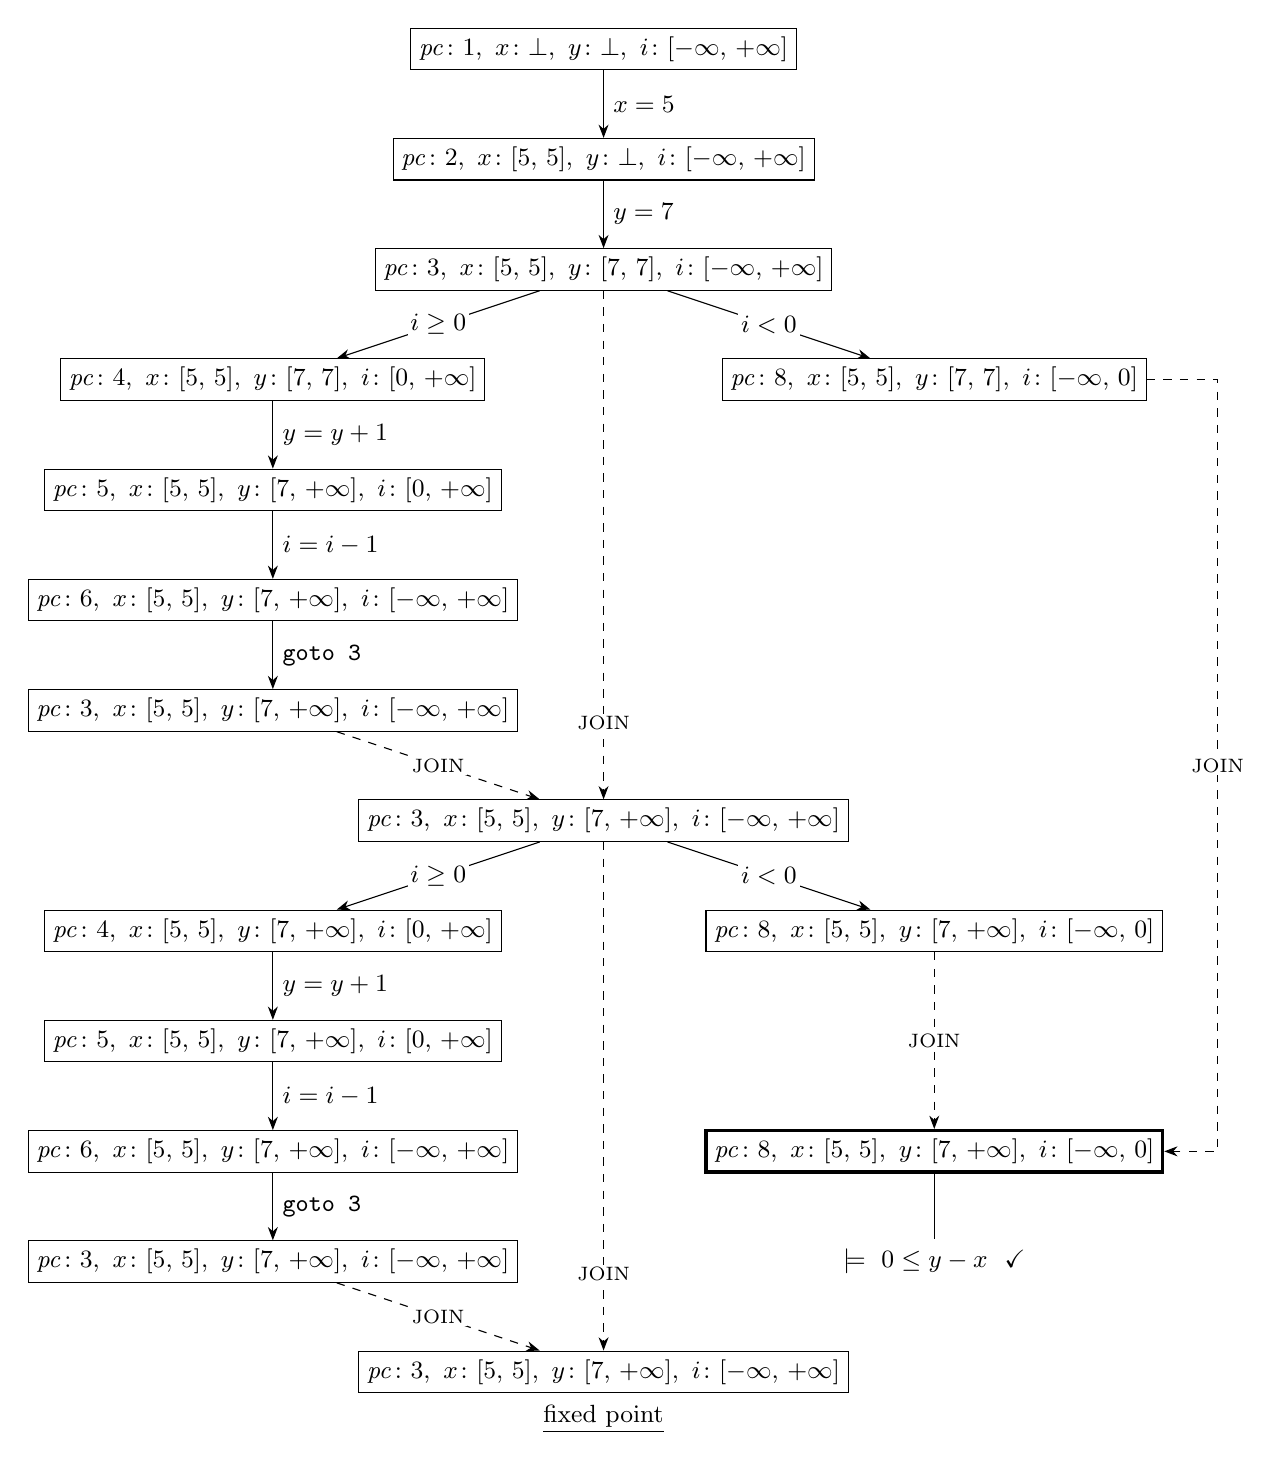
\begin{tikzpicture}[
    state/.style={draw, rectangle, align=center, inner sep=3pt, font=\small},
    instr/.style={-{Stealth}},
    meta/.style={-{Stealth}, dashed},
    lbl/.style={font=\small},
    mlbl/.style={font=\scriptsize, fill=white, inner sep=1pt}
  ]

  % before the loop
  \node[state] (s1)  at (0,0)       {\sti{1}{\bot}{\bot}{\itv{\ninf}{\pinf}}};
  \node[state] (s2)  at (0,-1.4)    {\sti{2}{\itv{5}{5}}{\bot}{\itv{\ninf}{\pinf}}};
  \node[state] (s3)  at (0,-2.8)    {\sti{3}{\itv{5}{5}}{\itv{7}{7}}{\itv{\ninf}{\pinf}}};

  % loop iteration 1
  \node[state] (s4)  at (-4.2,-4.2) {\sti{4}{\itv{5}{5}}{\itv{7}{7}}{\itv{0}{\pinf}}};
  \node[state] (s8a) at (4.2,-4.2)  {\sti{8}{\itv{5}{5}}{\itv{7}{7}}{\itv{\ninf}{0}}};
  \node[state] (s5)  at (-4.2,-5.6) {\sti{5}{\itv{5}{5}}{\itv{7}{\pinf}}{\itv{0}{\pinf}}};
  \node[state] (s6)  at (-4.2,-7)   {\sti{6}{\itv{5}{5}}{\itv{7}{\pinf}}{\itv{\ninf}{\pinf}}};
  \node[state] (s3b) at (-4.2,-8.4) {\sti{3}{\itv{5}{5}}{\itv{7}{\pinf}}{\itv{\ninf}{\pinf}}};
  \node[state] (s3j) at (0,-9.8)    {\sti{3}{\itv{5}{5}}{\itv{7}{\pinf}}{\itv{\ninf}{\pinf}}};

  % loop iteration 2
  \node[state] (t4)  at (-4.2,-11.2) {\sti{4}{\itv{5}{5}}{\itv{7}{\pinf}}{\itv{0}{\pinf}}};
  \node[state] (s8b) at (4.2,-11.2)  {\sti{8}{\itv{5}{5}}{\itv{7}{\pinf}}{\itv{\ninf}{0}}};
  \node[state] (t5)  at (-4.2,-12.6) {\sti{5}{\itv{5}{5}}{\itv{7}{\pinf}}{\itv{0}{\pinf}}};
  \node[state] (t6)  at (-4.2,-14)   {\sti{6}{\itv{5}{5}}{\itv{7}{\pinf}}{\itv{\ninf}{\pinf}}};
  \node[state] (t3b) at (-4.2,-15.4) {\sti{3}{\itv{5}{5}}{\itv{7}{\pinf}}{\itv{\ninf}{\pinf}}};
  \node[state] (s3f) at (0,-16.8)    {\sti{3}{\itv{5}{5}}{\itv{7}{\pinf}}{\itv{\ninf}{\pinf}}};
  \node[lbl, below=1pt] at (s3f.south) {\underline{fixed point}};

  % exit
  \node[state, very thick] (s8) at (4.2,-14) {\sti{8}{\itv{5}{5}}{\itv{7}{\pinf}}{\itv{\ninf}{0}}};
  \node[lbl] (chk) at (4.2,-15.4) {$\models\ 0 \le y - x$ \ \checkmark};

  % edges before the loop
  \draw[instr] (s1) -- node[lbl, right] {$x = 5$} (s2);
  \draw[instr] (s2) -- node[lbl, right] {$y = 7$} (s3);

  % edges loop iteration 1
  \draw[instr] (s3) -- node[mlbl, font=\small]  {$i \ge 0$} (s4);
  \draw[instr] (s3) -- node[mlbl, font=\small] {$i < 0$}   (s8a);
  \draw[instr] (s4) -- node[lbl, right] {$y = y + 1$} (s5);
  \draw[instr] (s5) -- node[lbl, right] {$i = i - 1$} (s6);
  \draw[instr] (s6) -- node[lbl, right] {\texttt{goto 3}} (s3b);
  \draw[meta]  (s3b) -- node[mlbl] {JOIN} (s3j);
  \draw[meta]  (s3)  -- node[mlbl, pos=0.85] {JOIN} (s3j);

  % edges loop iteration 2
  \draw[instr] (s3j) -- node[mlbl, font=\small]  {$i \ge 0$} (t4);
  \draw[instr] (s3j) -- node[mlbl, font=\small] {$i < 0$}   (s8b);
  \draw[instr] (t4) -- node[lbl, right] {$y = y + 1$} (t5);
  \draw[instr] (t5) -- node[lbl, right] {$i = i - 1$} (t6);
  \draw[instr] (t6) -- node[lbl, right] {\texttt{goto 3}} (t3b);
  \draw[meta]  (t3b) -- node[mlbl] {JOIN} (s3f);
  \draw[meta]  (s3j) -- node[mlbl, pos=0.85] {JOIN} (s3f);

  % edges exit
  \draw[meta]  (s8a.east) -- (7.8,-4.2) |- node[mlbl, pos=0.25] {JOIN} (s8.east);
  \draw[meta]  (s8b) -- node[mlbl] {JOIN} (s8);
  \draw (s8) -- (chk);
\end{tikzpicture}\end{fitbox}
\end{center}

\paragraph{Check.}
At line 8, $x \in \itv{5}{5}$ and $y \in \itv{7}{\pinf}$, so
$y - x \in \itv{2}{\pinf}$ and $0 \le y - x$ holds. Hence $P_{\INTp} \models (0 \le y - x)$
\checkmark, and \texttt{Foo} is verified without widening.

The analysis terminates because $\INTp$ has finite height: the state at line 3 can only grow
finitely often. It is precise enough because the lower bound $7$ of $y$ is a threshold and
$y$ only grows, so the lower bound is never lost. Only the upper bound jumps directly to
$\pinf$, which is what widening would have done.

\subsection*{Height of $\INTp$}

In a strictly increasing chain $\bot \sqsubset e_1 \sqsubset e_2 \sqsubset \dots$, each step
after $e_1$ moves the lower bound down or the upper bound up by at least one position in the
ordered set $\ninf < 0 < 5 < 7 < \pinf$.
\begin{itemize}
  \item The longest chains start in a singleton $[k,k]$ with $k \in \{0, 5, 7\}$ (position
        $j \in \{1,2,3\}$, counting from $0$).
  \item The lower bound can move down at most $j$ times and the upper bound can move up at
        most $4 - j$ times, i.e.\ 4 steps in total.
  \item Together with the step $\bot \sqsubset [k,k]$, every chain has at most 5 steps.
\end{itemize}
This bound is reached, e.g.\ by
\[
  \bot \sqsubset \itv{5}{5} \sqsubset \itv{5}{7} \sqsubset \itv{5}{\pinf}
       \sqsubset \itv{0}{\pinf} \sqsubset \itv{\ninf}{\pinf}.
\]
So the \textbf{height of $\INTp$ is 5} (the longest chain has 6 elements).

\subsection*{A program verified with standard intervals but not with $\INTp$}

\begin{lstlisting}
void P() {
    int x = 1;
    assert(x <= 1);
}
\end{lstlisting}

\begin{center}
\begin{fitbox}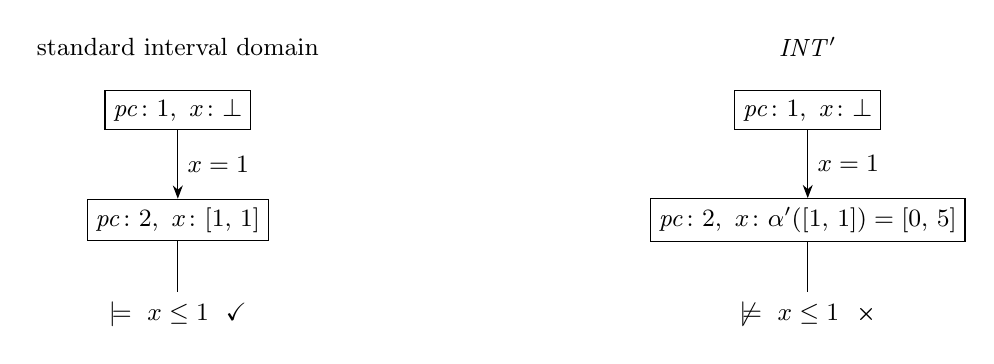
\begin{tikzpicture}[
    state/.style={draw, rectangle, align=center, inner sep=3pt, font=\small},
    instr/.style={-{Stealth}},
    lbl/.style={font=\small}
  ]
  % standard interval domain
  \node[lbl] at (-4,0.8) {standard interval domain};
  \node[state] (a1) at (-4,0)    {$\mathit{pc}\colon 1,\ x\colon \bot$};
  \node[state] (a2) at (-4,-1.4) {$\mathit{pc}\colon 2,\ x\colon \itv{1}{1}$};
  \node[lbl]   (ac) at (-4,-2.6) {$\models\ x \le 1$ \ \checkmark};
  \draw[instr] (a1) -- node[lbl, right] {$x = 1$} (a2);
  \draw (a2) -- (ac);

  % INT'
  \node[lbl] at (4,0.8) {$\INTp$};
  \node[state] (b1) at (4,0)    {$\mathit{pc}\colon 1,\ x\colon \bot$};
  \node[state] (b2) at (4,-1.4) {$\mathit{pc}\colon 2,\ x\colon \alpha'(\itv{1}{1}) = \itv{0}{5}$};
  \node[lbl]   (bc) at (4,-2.6) {$\not\models\ x \le 1$ \ \texttimes};
  \draw[instr] (b1) -- node[lbl, right] {$x = 1$} (b2);
  \draw (b2) -- (bc);
\end{tikzpicture}\end{fitbox}
\end{center}

\begin{itemize}
  \item \textbf{Standard interval domain:} $x = 1$ gives $x \in \itv{1}{1}$, so $x \le 1$
        holds and the assertion is verified. The program has no loop, so no widening is needed.
  \item \textbf{$\INTp$:} $1 \notin K$, so the constant is over-approximated as
        $\alpha'(\itv{1}{1}) = \itv{0}{5}$. This interval contains values $> 1$ (e.g.\ $2$),
        so the assertion cannot be verified. This is a false alarm caused by the coarser
        domain.
\end{itemize}

\end{document}
